\begin{figure*}[ht]
    \centering
    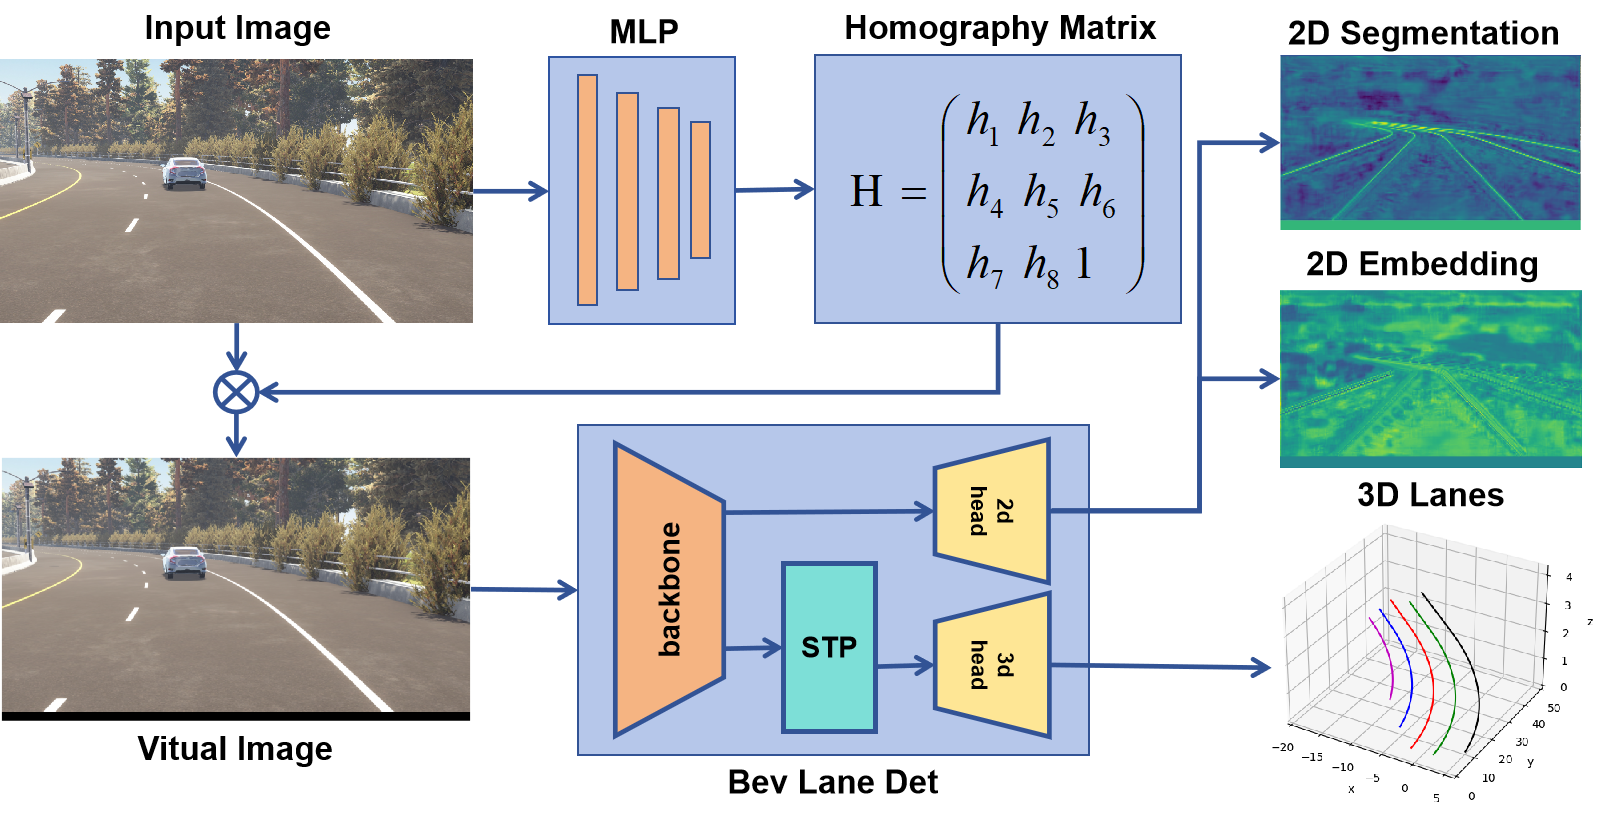
\includegraphics[height=0.3\textheight]{asset/structure3} %width=1\linewidth
    \caption{Overview of the framework}
    \label{fig:overview}
\end{figure*}

\section{Methods}
\label{sec:methods}
%Fig.\ref{fig:overview} shows the overview of our entire lane detection framework.
An overview of our entire lane detection framework is illustrated in Fig.\ref{fig:overview}.
Our approach takes a single image captured by a front camera mounted on the vehicle as input.
The image is projected to the virtual camera view with the homography
matrix generated by MLP network \cite{tang2022image},
which aims to unify the in/extrinsic parameters of front-facing cameras in different vehicles.

We use ResNet18 and ResNet34 \cite{he2016deep} as our backbone to extract virtual camera view image features, called front-view features.
Spatial Transformation Pyramid \cite{wang2023bev} transform the front-view features into BEV features.
Then, lanes are predicted on the BEV view. We predict the confidence of each cell, the embedding used for clustering,
the offset from the center of the cell to the lane in the y-direction, and the height.
we added the front view lane detection header as an
auxiliary supervision to improve backbone's ability to extract front view features
and supervise the homography matrix estimation network's training.

\subsection{Homography Transformation}
Homography matrix is the simplest kind of transformation that describes the 2D relationship between two images.
It can be mathematically described by a 3D transformation in a homogeneous coordinates space and can be expressed as:

\[
\left[ \begin{matrix}
   x'  \\
   y'  \\
   1
\end{matrix} \right]
=
H\left[ \begin{matrix}
   x  \\
   y  \\
   1
\end{matrix} \right]
=
\left[ \begin{matrix}
h_1 & h_2 & h_3  \\
h_4 & h_5 & h_6  \\
h_7 & h_8 & h_9  \\
\end{matrix} \right]
\left[ \begin{matrix}
x  \\
y  \\
1
\end{matrix} \right]
\]
where H denotes the homography matrix $H \in R^{3\times 3}$ between two two-dimensional planes,
which allows us to transform images from one view to another by multiplying the homography matrix.
$(x, y)$ is the principle point in the image plane, and $(x', y')$ is the corresponding point in the target image.

Homography matrix is usually parameterized by the elements of a 3×3 matrix,
but it has only 8 degrees of freedom, and a simple way to do this is to hardcode $h_9=1$.
We take the original image as input and use network to estimate the eight parameters.

\begin{figure}[hb]
    \centering
    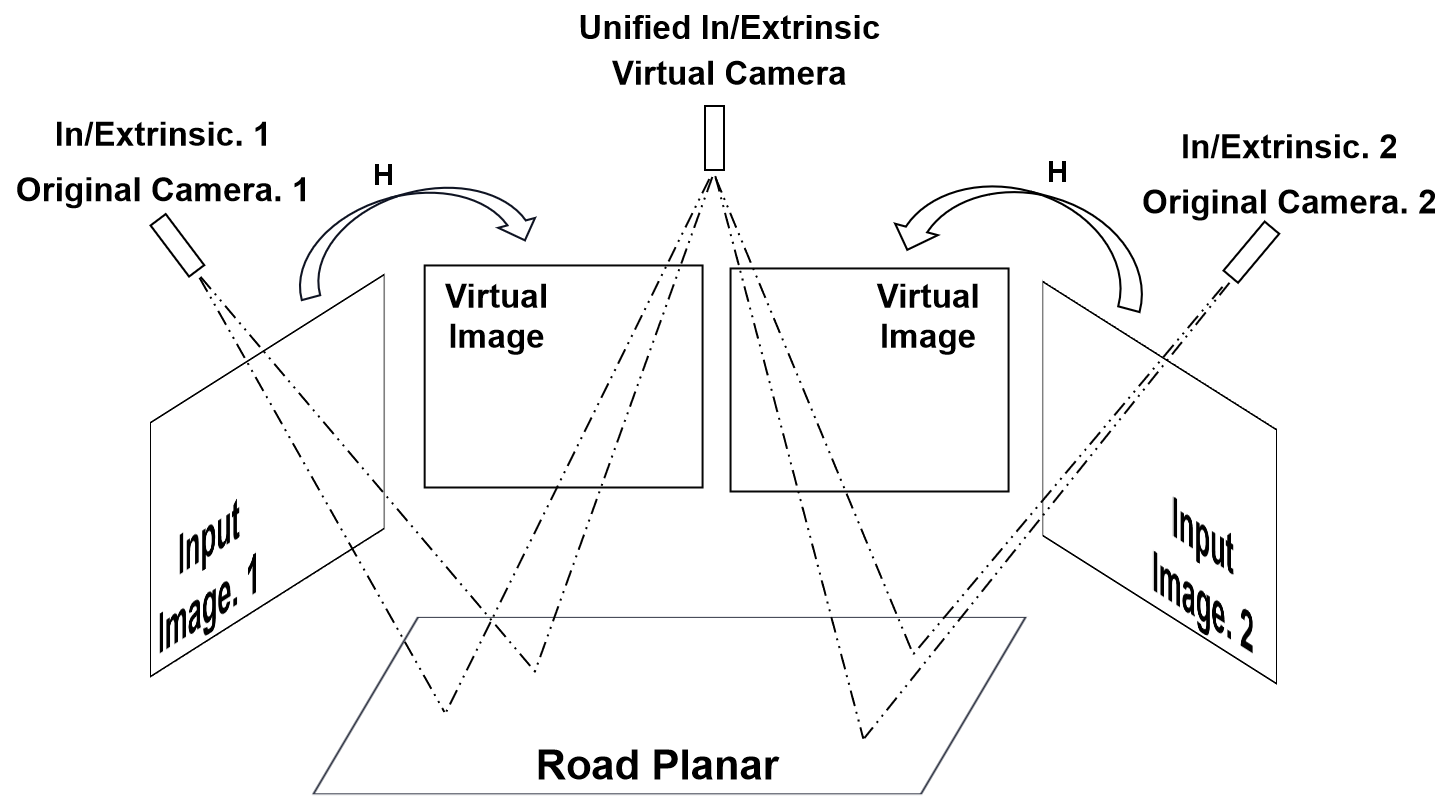
\includegraphics[width=\linewidth]{asset/virtual_camera}
    \caption{Virtual Camera}
    \label{fig:Virtual Camera}
\end{figure}

\begin{table}[htb]
    \caption{FVHNet network architecture.}\label{tab:FVHNet network architecture}
    \renewcommand{\arraystretch}{1.2}
    \center
    \begin{tabular}{|c|c|c|c|}% 其中,tabular是表格内容的环境;c表示centering,即文本格式居中;c的个数代表列的个数
        \hline %[2pt]设置线宽 %[2pt]设置线宽
        Type & Filters & Size/Stride & Output \\
        \hline %[2pt]设置线宽
        Conv+BN+ReLU   &    6  &   3x3      & 576x1024  \\
        \hline
        Conv+BN+ReLU   &    12  &   3x3      & 576x1024  \\
        \hline
        Maxpool        &        &   2x2/2    & 288x512  \\
        \hline
        Conv+BN+ReLU   &    24  &   3x3      & 288x512  \\
        \hline
        Conv+BN+ReLU   &    48  &   3x3      & 288x512  \\
        \hline
        Maxpool        &        &   2x2/2    & 144x256  \\
        \hline
        Conv+BN+ReLU   &    96  &   3x3      & 144x256  \\
        \hline
        Conv+BN+ReLU   &    192  &   3x3      & 144x256  \\
        \hline
        Maxpool        &        &   2x2/2    & 72x128  \\
        \hline
        Conv+BN+ReLU   &    128  &   3x3      & 72x128 \\
        \hline
        Conv+BN+ReLU   &    128  &   3x3      & 72x128 \\
        \hline
        Maxpool        &        &   2x2/2    & 36x64  \\
        \hline
        Conv+BN+ReLU   &    128  &   3x3      & 36x64  \\
        \hline
        Conv+BN+ReLU   &    96  &   3x3      & 36x64  \\
        \hline
        Maxpool        &        &   2x2/2    & 18x32  \\
        \hline
        Conv+BN+ReLU   &    64  &   3x3      & 18x32  \\
        \hline
        Conv+BN+ReLU   &    32  &   3x3      & 18x32  \\
        \hline
        Linear+BN+ReLU &        &   1x1      & 1024  \\
        \hline
        Linear         &        &   1x1      & 8  \\
        \hline
    \end{tabular}
\end{table}

\subsection{FVHNet}
\label{subsec:FVHNet}
Different cameras mounted on the vehicle have different internal/external parameters,
which have a significant effect on the 3D lane results.
As shown in Fig.\ref{fig:Virtual Camera},
we can unify the internal/external parameters of different cameras by creating a virtual camera.
Therefore, we need transform front-view images to virtual camera images by homography matrix,
which can guarantee the consistency of the spatial relationship among cameras.
However, if a fixed transformation matrix is employed, the projection becomes less accurate.
Towards the issue, we train FVHNet, a simple and efficient network, to output certain crucial parameters in the homography transformation.
The network architecture of FVHNet is constructed out of consecutive blocks of 3x3 convolutions, batchnorm and ReLUs.
The dimension is decreased using max pooling layers, and in the end 2 fully-connected layers are added.
See Tab.\ref{tab:FVHNet network architecture} for the complete network structure.

\subsection{FVH Loss}
\label{subsec:FVH Loss}
In order to improve the MLP network's ability to extract homography matrix parameters and backbone's ability to extract front view features,
a front view lane detection header was added as an auxiliary supervision.
Based on this front view lane detection head, we propose the homography loss function.
The input image is converted to a virtual camera image by homography matrix $H$.
Then, the front-view features are obtained by backbone,
and the front-view lane detection head gets the segmentation and embedding results,
which are transformed back to the input camera view by the inverse matrix $H^{-1}$ of the homography matrix.
As shown in Fig.\ref{fig:FVH Loss Image}, FVHLoss includes lane segmentation loss and lane embedding loss,
referred to LaneNet~\cite{neven2018towards}.It is defined as follows,
\[
L_{h}=\lambda_{seg}^h L_{seg}^h + \lambda_{emb}^h L_{emb}^h + \lambda_{hm}^h L_{hm}^h
\]
where $L_{seg}^h$ denotes lane segmentation loss, $L_{emb}^h$ denotes lane embedding loss,
and $L_{hm}^h$ denotes SmoothL1 loss between predicted and ground truth homography matrix.
The ground truth homography matrix is calculated according to the camera intrinsic parameters and extrinsic parameters
provided by the current camera and the in/extrinsic parameters of the Virtual Camera which are derived from the mean value of the in/extrinsic
parameters of the training dataset.
\begin{figure}[htb]
    \centering
    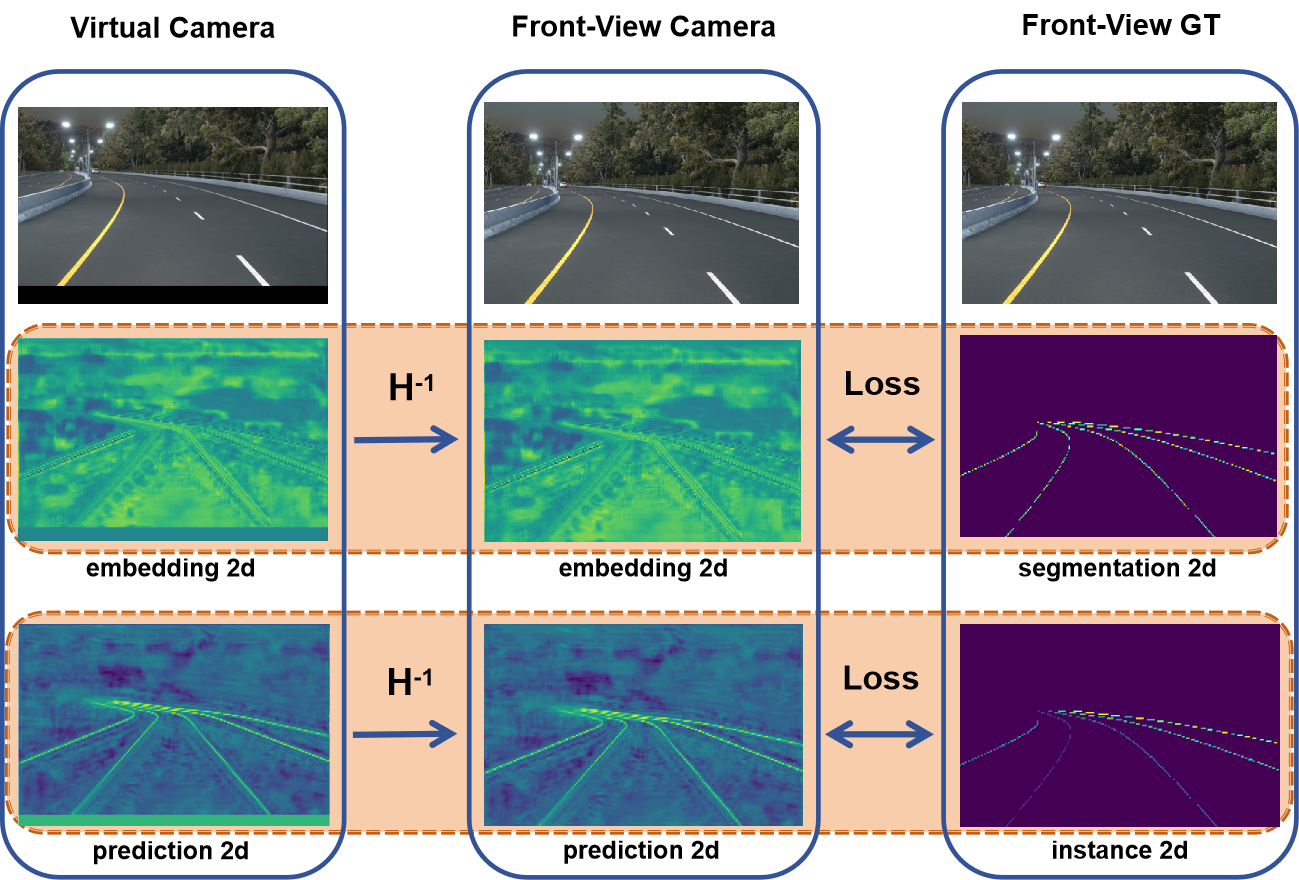
\includegraphics[width=0.9\linewidth]{asset/loss4}
    \caption{FVH Loss}
    \label{fig:FVH Loss Image}
\end{figure}
